%%%%%%%%%%%%%%%%%%%%%%%%%%%%%%%%%%%%%%%%%
% University Assignment Title Page 
% LaTeX Template
% Version 1.0 (27/12/12)
%
% This template has been downloaded from:
% http://www.LaTeXTemplates.com
%
% Original author:
% WikiBooks (http://en.wikibooks.org/wiki/LaTeX/Title_Creation)
%
% License:
% CC BY-NC-SA 3.0 (http://creativecommons.org/licenses/by-nc-sa/3.0/)
% 
% Instructions for using this template:
% This title page is capable of being compiled as is. This is not useful for 
% including it in another document. To do this, you have two options: 
%
% 1) Copy/paste everything between \begin{document} and \end{document} 
% starting at \begin{titlepage} and paste this into another LaTeX file where you 
% want your title page.
% OR
% 2) Remove everything outside the \begin{titlepage} and \end{titlepage} and 
% move this file to the same directory as the LaTeX file you wish to add it to. 
% Then add %%%%%%%%%%%%%%%%%%%%%%%%%%%%%%%%%%%%%%%%%
% University Assignment Title Page 
% LaTeX Template
% Version 1.0 (27/12/12)
%
% This template has been downloaded from:
% http://www.LaTeXTemplates.com
%
% Original author:
% WikiBooks (http://en.wikibooks.org/wiki/LaTeX/Title_Creation)
%
% License:
% CC BY-NC-SA 3.0 (http://creativecommons.org/licenses/by-nc-sa/3.0/)
% 
% Instructions for using this template:
% This title page is capable of being compiled as is. This is not useful for 
% including it in another document. To do this, you have two options: 
%
% 1) Copy/paste everything between \begin{document} and \end{document} 
% starting at \begin{titlepage} and paste this into another LaTeX file where you 
% want your title page.
% OR
% 2) Remove everything outside the \begin{titlepage} and \end{titlepage} and 
% move this file to the same directory as the LaTeX file you wish to add it to. 
% Then add %%%%%%%%%%%%%%%%%%%%%%%%%%%%%%%%%%%%%%%%%
% University Assignment Title Page 
% LaTeX Template
% Version 1.0 (27/12/12)
%
% This template has been downloaded from:
% http://www.LaTeXTemplates.com
%
% Original author:
% WikiBooks (http://en.wikibooks.org/wiki/LaTeX/Title_Creation)
%
% License:
% CC BY-NC-SA 3.0 (http://creativecommons.org/licenses/by-nc-sa/3.0/)
% 
% Instructions for using this template:
% This title page is capable of being compiled as is. This is not useful for 
% including it in another document. To do this, you have two options: 
%
% 1) Copy/paste everything between \begin{document} and \end{document} 
% starting at \begin{titlepage} and paste this into another LaTeX file where you 
% want your title page.
% OR
% 2) Remove everything outside the \begin{titlepage} and \end{titlepage} and 
% move this file to the same directory as the LaTeX file you wish to add it to. 
% Then add %%%%%%%%%%%%%%%%%%%%%%%%%%%%%%%%%%%%%%%%%
% University Assignment Title Page 
% LaTeX Template
% Version 1.0 (27/12/12)
%
% This template has been downloaded from:
% http://www.LaTeXTemplates.com
%
% Original author:
% WikiBooks (http://en.wikibooks.org/wiki/LaTeX/Title_Creation)
%
% License:
% CC BY-NC-SA 3.0 (http://creativecommons.org/licenses/by-nc-sa/3.0/)
% 
% Instructions for using this template:
% This title page is capable of being compiled as is. This is not useful for 
% including it in another document. To do this, you have two options: 
%
% 1) Copy/paste everything between \begin{document} and \end{document} 
% starting at \begin{titlepage} and paste this into another LaTeX file where you 
% want your title page.
% OR
% 2) Remove everything outside the \begin{titlepage} and \end{titlepage} and 
% move this file to the same directory as the LaTeX file you wish to add it to. 
% Then add \input{./title_page_1.tex} to your LaTeX file where you want your
% title page.
%t
%%%%%%%%%%%%%%%%%%%%%%%%%%%%%%%%%%%%%%%%%
\title{Báo cáo đồ án cuối kỳ}
%----------------------------------------------------------------------------------------
%	PACKAGES AND OTHER DOCUMENT CONFIGURATIONS
%----------------------------------------------------------------------------------------

\documentclass[12pt]{article}
\usepackage[T5]{fontenc}
\usepackage[utf8]{inputenc}
\usepackage[vietnamese,english]{babel}
\usepackage{amsmath}
\usepackage{graphicx}
\usepackage[colorinlistoftodos]{todonotes}
\usepackage{listings}
\usepackage{hyperref}
\hypersetup{
    colorlinks=true,
    linkcolor=blue,
    filecolor=magenta,      
    urlcolor=cyan,
}


\begin{document}

\begin{titlepage}

\newcommand{\HRule}{\rule{\linewidth}{0.5mm}} % Defines a new command for the horizontal lines, change thickness here

\center % Center everything on the page
 
%----------------------------------------------------------------------------------------
%	HEADING SECTIONS
%----------------------------------------------------------------------------------------

\textsc{\LARGE Đại học Khoa học tự nhiên}\\[1.5cm] % Name of your university/college
\textsc{\Large Ngành hệ thống thông tin}\\[0.5cm] % Major heading such as course name
\textsc{\large Môn học: Máy học thống kê }\\[0.5cm] % Minor heading such as course title

%----------------------------------------------------------------------------------------
%	TITLE SECTION
%----------------------------------------------------------------------------------------

\HRule \\[0.4cm]
{ \huge \bfseries Báo cáo đồ án ứng dụng Yolo}\\[0.4cm] % Title of your document
\HRule \\[1.5cm]
 
%----------------------------------------------------------------------------------------
%	AUTHOR SECTION
%----------------------------------------------------------------------------------------

\begin{minipage}{0.4\textwidth}
\begin{flushleft} \large
\emph{Học viên:}\\
Thái Thiện -- 17C 12 031 % Your name
\end{flushleft}
\end{minipage}
~
\begin{minipage}{0.4\textwidth}
\begin{flushright} \large
\emph{Giảng viên:} \\
TS. Ngô Minh Nhựt % Supervisor's Name
\end{flushright}
\end{minipage}\\[2cm]

% If you don't want a supervisor, uncomment the two lines below and remove the section above
%\Large \emph{Author:}\\
%John \textsc{Smith}\\[3cm] % Your name

%----------------------------------------------------------------------------------------
%	DATE SECTION
%----------------------------------------------------------------------------------------

% I don't want day because it is English
% {\large \today}\\[2cm] % Date, change the \today to a set date if you want to be precise

%----------------------------------------------------------------------------------------
%	LOGO SECTION
%----------------------------------------------------------------------------------------


\includegraphics{logo/rsz_3logo-khtn.png}\\[1cm] % Include a department/university logo - this will require the graphicx package
 
%----------------------------------------------------------------------------------------

\vfill % Fill the rest of the page with whitespace

\end{titlepage}


\section{Yolo}

Trang chủ: \url{https://pjreddie.com/darknet/yolo/} 

YOLO - You Only look once - là hệ thống nhận dạng vật thể thời gian thực.

Trong đồ án này, chúng tôi sử dụng YOLOv3 

\section{Cài đặt Yolo để nhận dạng ảnh}

\subsection{Mã nguồn của tác giả YOLO}

Tác giả có hướng dẫn cách cài đặt YOLO tại trang chủ  \url{https://pjreddie.com/darknet/yolo/}. Máy tính chúng tôi dùng sử dụng hệ điều hành Ubuntu 16.04 LTS. 

Cài những thứ cần thiết để build với dòng lệnh ở lstlisting \ref{lst:buildessential}.

\begin{lstlisting}[caption={Cài những gói cần thiết để build}, label={lst:buildessential}, language=bash]
sudo apt-get build-essential
sudo apt-get install git
\end{lstlisting}

Sau đó tải mã nguồn từ Github \footnote{\url{https://github.com/pjreddie/darknet}} về build với các dòng lệnh sau (lstlisting \ref{lst:buildyolo})


\begin{lstlisting}[caption={Tải và build mã nguồn}, label={lst:buildyolo}, language=bash]
git clone https://github.com/pjreddie/darknet   
cd darknet 
make  
\end{lstlisting}

Sau đó tải model (loại lớn) \footnote{\url{https://pjreddie.com/media/files/yolov3.weights}}  huấn luyện kèm với config \footnote{\url{https://github.com/pjreddie/darknet/blob/master/cfg/yolov3.cfg}}. Ngoài ra còn có loại nhỏ (tiny) \footnote{\url{https://pjreddie.com/media/files/yolov3-tiny.weights}} và config nhỏ \footnote{\url{https://github.com/pjreddie/darknet/blob/master/cfg/yolov3-tiny.cfg}}. 

Sau đó, chạy theo ví dụ của tác giả (lstlisting \ref{lst:runexample}) hoặc theo cú pháp (lstlisting \ref{lst:runsyntax})

\begin{lstlisting}[caption={ví dụ chạy nhận diện vật thể}, label={lst:runexample}, language=bash]
./darknet detect cfg/yolov3.cfg yolov3.weights data/dog.jpg
\end{lstlisting}


\begin{lstlisting}[caption={ví dụ chạy nhận diện vật thể}, label={lst:runsyntax}, language=bash]
./darknet detect <config path> <weight path> <input image>
\end{lstlisting}


\subsection{Cài đặt YOLO bằng python}

Các tập tin python tác giả cung cấp có vẻ không tương thích với đoạn mã c++ mà chúng tôi build được ở bước trên. Vì vậy chúng tôi quyết định tìm kiếm giải pháp khác. Chúng tôi kế thừa từ mã nguồn của Ayoosh Kathuria \footnote{\url{https://github.com/ayooshkathuria/pytorch-yolo-v3}} và cải tiến cho phù hợp với nhu cầu \footnote{\url{https://github.com/ttpro1995/pytorch-yolo-v3}}.  

Yêu cầu: 
\begin{itemize}
\item python 3.6
\item Anaconda \footnote{\url{https://www.anaconda.com/download/}}
\item Pytorch \footnote{\url{https://pytorch.org/}}
\item opencv-python 
\end{itemize}

\subsubsection{Yolo Wrapper - Một lớp (class) dễ sử dụng}

Chúng tôi xây dựng một lớp YoloWrapper bao gồm hàm tạo và hàm predict để tiện việc gắn vào ứng dụng 

\paragraph{Khởi tạo}
Bước khởi tạo cần làm 3 việc: nạp danh sách lớp (từ coco.names), nạp mô hình trọng số và config. 

\paragraph{Dự đoán}
Bước dự đoán thực hiện các bước sau 

\begin{itemize}
\item Tiền xử lý: biến đổi ảnh đầu vào cho phù hợp với chiều của mạng yolo (416) 
\item Dự đoán: bỏ ma trận hình ảnh sau khi tiền xử lý vào mô hình yolo 
\item Ghi kết quả: từ kết quả dự đoán, ghi kết quả theo dạng [hình trong batch, tọa độ khung 1, tọa độ khung 2, tọa độ khung 3, tọa độ khung 4, xxx, độ tự tin, số thứ tự của tên vật thể]. Bước ghi kết quả chỉ ghi lại kết quả có độ tự tin lớn hơn threshold 
\item Scale: cái khung ở bước ghi kết quả dựa và cái hình sau khi đã biến đổi cho phù hợp với mô hình. Ta cần biến đổ nó trở lại đúng với ảnh gốc để vẽ vào ảnh gốc 
\item Vẽ khung dự đoán và tên vật thể vào ảnh gốc và trả về kết quả 
\end{itemize} 


\subsubsection{Mẫu thiết kế Singleton}

\section{Dùng Django để tạo ứng dụng web cho yolo}





Trích dẫn hình \ref{fig:node} trong đoạn chữ. 

% % Commands to include a figure:
\begin{figure}[h]
\centering

\includegraphics[width=0.5\textwidth]{image/node.PNG}
\caption{\label{fig:node} Nút}
\end{figure}


% chuong 3
\section{Chèn đoạn code}


ví dụ code \ref{lst:vdcode} là code python 


\begin{lstlisting}[caption={Đoạn code}, label={lst:vdcode}, language=python]
s = "I am Pusheen the cat"
print(s)
\end{lstlisting}

ví dụ trích dẫn \cite{robinson2013graph}


\bibliographystyle{IEEEtran}
\bibliography{bib}

%%%%%%%%%%%%%%%%%%%%%%%%%%%%%%%%%%%%%%%%%%%%%%%%%%%%
% Comments can be added to the margins of the document using the \todo{Here's a comment in the margin!} todo command, as shown in the example on the right. You can also add inline comments too:

% \todo[inline, color=green!40]{This is an inline comment.}



% \subsection{Tables and Figures}

% Use the table and tabular commands for basic tables --- see Table~\ref{tab:widgets}, for example. You can upload a figure (JPEG, PNG or PDF) using the files menu. To include it in your document, use the includegraphics command as in the code for Figure~\ref{fig:frog} below.

% % % Commands to include a figure:
% % \begin{figure}
% % \centering
% % 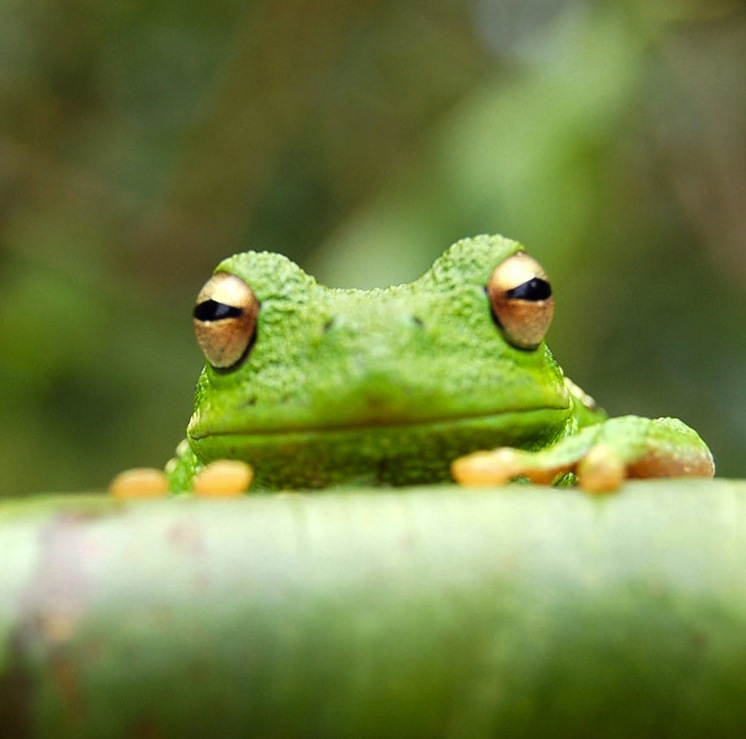
\includegraphics[width=0.5\textwidth]{frog.jpg}
% % \caption{\label{fig:frog}This is a figure caption.}
% % \end{figure}

% % \begin{table}
% % \centering
% % \begin{tabular}{l|r}
% % Item & Quantity \\\hline
% % Widgets & 42 \\
% % Gadgets & 13
% % \end{tabular}
% % \caption{\label{tab:widgets}An example table.}
% % \end{table}

% \subsection{Mathematics}

% \LaTeX{} is great at typesetting mathematics. Let $X_1, X_2, \ldots, X_n$ be a sequence of independent and identically distributed random variables with $\text{E}[X_i] = \mu$ and $\text{Var}[X_i] = \sigma^2 < \infty$, and let
% $$S_n = \frac{X_1 + X_2 + \cdots + X_n}{n}
%       = \frac{1}{n}\sum_{i}^{n} X_i$$
% denote their mean. Then as $n$ approaches infinity, the random variables $\sqrt{n}(S_n - \mu)$ converge in distribution to a normal $\mathcal{N}(0, \sigma^2)$.

% \subsection{Lists}

% You can make lists with automatic numbering \dots

% \begin{enumerate}
% \item Like this,
% \item and like this.
% \end{enumerate}
% \dots or bullet points \dots
% \begin{itemize}
% \item Like this,
% \item and like this.
% \end{itemize}

% We hope you find write\LaTeX\ useful, and please let us know if you have any feedback using the help menu above.

\end{document} to your LaTeX file where you want your
% title page.
%t
%%%%%%%%%%%%%%%%%%%%%%%%%%%%%%%%%%%%%%%%%
\title{Báo cáo đồ án cuối kỳ}
%----------------------------------------------------------------------------------------
%	PACKAGES AND OTHER DOCUMENT CONFIGURATIONS
%----------------------------------------------------------------------------------------

\documentclass[12pt]{article}
\usepackage[T5]{fontenc}
\usepackage[utf8]{inputenc}
\usepackage[vietnamese,english]{babel}
\usepackage{amsmath}
\usepackage{graphicx}
\usepackage[colorinlistoftodos]{todonotes}
\usepackage{listings}
\usepackage{hyperref}
\hypersetup{
    colorlinks=true,
    linkcolor=blue,
    filecolor=magenta,      
    urlcolor=cyan,
}


\begin{document}

\begin{titlepage}

\newcommand{\HRule}{\rule{\linewidth}{0.5mm}} % Defines a new command for the horizontal lines, change thickness here

\center % Center everything on the page
 
%----------------------------------------------------------------------------------------
%	HEADING SECTIONS
%----------------------------------------------------------------------------------------

\textsc{\LARGE Đại học Khoa học tự nhiên}\\[1.5cm] % Name of your university/college
\textsc{\Large Ngành hệ thống thông tin}\\[0.5cm] % Major heading such as course name
\textsc{\large Môn học: Máy học thống kê }\\[0.5cm] % Minor heading such as course title

%----------------------------------------------------------------------------------------
%	TITLE SECTION
%----------------------------------------------------------------------------------------

\HRule \\[0.4cm]
{ \huge \bfseries Báo cáo đồ án ứng dụng Yolo}\\[0.4cm] % Title of your document
\HRule \\[1.5cm]
 
%----------------------------------------------------------------------------------------
%	AUTHOR SECTION
%----------------------------------------------------------------------------------------

\begin{minipage}{0.4\textwidth}
\begin{flushleft} \large
\emph{Học viên:}\\
Thái Thiện -- 17C 12 031 % Your name
\end{flushleft}
\end{minipage}
~
\begin{minipage}{0.4\textwidth}
\begin{flushright} \large
\emph{Giảng viên:} \\
TS. Ngô Minh Nhựt % Supervisor's Name
\end{flushright}
\end{minipage}\\[2cm]

% If you don't want a supervisor, uncomment the two lines below and remove the section above
%\Large \emph{Author:}\\
%John \textsc{Smith}\\[3cm] % Your name

%----------------------------------------------------------------------------------------
%	DATE SECTION
%----------------------------------------------------------------------------------------

% I don't want day because it is English
% {\large \today}\\[2cm] % Date, change the \today to a set date if you want to be precise

%----------------------------------------------------------------------------------------
%	LOGO SECTION
%----------------------------------------------------------------------------------------


\includegraphics{logo/rsz_3logo-khtn.png}\\[1cm] % Include a department/university logo - this will require the graphicx package
 
%----------------------------------------------------------------------------------------

\vfill % Fill the rest of the page with whitespace

\end{titlepage}


\section{Yolo}

Trang chủ: \url{https://pjreddie.com/darknet/yolo/} 

YOLO - You Only look once - là hệ thống nhận dạng vật thể thời gian thực.

Trong đồ án này, chúng tôi sử dụng YOLOv3 

\section{Cài đặt Yolo để nhận dạng ảnh}

\subsection{Mã nguồn của tác giả YOLO}

Tác giả có hướng dẫn cách cài đặt YOLO tại trang chủ  \url{https://pjreddie.com/darknet/yolo/}. Máy tính chúng tôi dùng sử dụng hệ điều hành Ubuntu 16.04 LTS. 

Cài những thứ cần thiết để build với dòng lệnh ở lstlisting \ref{lst:buildessential}.

\begin{lstlisting}[caption={Cài những gói cần thiết để build}, label={lst:buildessential}, language=bash]
sudo apt-get build-essential
sudo apt-get install git
\end{lstlisting}

Sau đó tải mã nguồn từ Github \footnote{\url{https://github.com/pjreddie/darknet}} về build với các dòng lệnh sau (lstlisting \ref{lst:buildyolo})


\begin{lstlisting}[caption={Tải và build mã nguồn}, label={lst:buildyolo}, language=bash]
git clone https://github.com/pjreddie/darknet   
cd darknet 
make  
\end{lstlisting}

Sau đó tải model (loại lớn) \footnote{\url{https://pjreddie.com/media/files/yolov3.weights}}  huấn luyện kèm với config \footnote{\url{https://github.com/pjreddie/darknet/blob/master/cfg/yolov3.cfg}}. Ngoài ra còn có loại nhỏ (tiny) \footnote{\url{https://pjreddie.com/media/files/yolov3-tiny.weights}} và config nhỏ \footnote{\url{https://github.com/pjreddie/darknet/blob/master/cfg/yolov3-tiny.cfg}}. 

Sau đó, chạy theo ví dụ của tác giả (lstlisting \ref{lst:runexample}) hoặc theo cú pháp (lstlisting \ref{lst:runsyntax})

\begin{lstlisting}[caption={ví dụ chạy nhận diện vật thể}, label={lst:runexample}, language=bash]
./darknet detect cfg/yolov3.cfg yolov3.weights data/dog.jpg
\end{lstlisting}


\begin{lstlisting}[caption={ví dụ chạy nhận diện vật thể}, label={lst:runsyntax}, language=bash]
./darknet detect <config path> <weight path> <input image>
\end{lstlisting}


\subsection{Cài đặt YOLO bằng python}

Các tập tin python tác giả cung cấp có vẻ không tương thích với đoạn mã c++ mà chúng tôi build được ở bước trên. Vì vậy chúng tôi quyết định tìm kiếm giải pháp khác. Chúng tôi kế thừa từ mã nguồn của Ayoosh Kathuria \footnote{\url{https://github.com/ayooshkathuria/pytorch-yolo-v3}} và cải tiến cho phù hợp với nhu cầu \footnote{\url{https://github.com/ttpro1995/pytorch-yolo-v3}}.  

Yêu cầu: 
\begin{itemize}
\item python 3.6
\item Anaconda \footnote{\url{https://www.anaconda.com/download/}}
\item Pytorch \footnote{\url{https://pytorch.org/}}
\item opencv-python 
\end{itemize}

\subsubsection{Yolo Wrapper - Một lớp (class) dễ sử dụng}

Chúng tôi xây dựng một lớp YoloWrapper bao gồm hàm tạo và hàm predict để tiện việc gắn vào ứng dụng 

\paragraph{Khởi tạo}
Bước khởi tạo cần làm 3 việc: nạp danh sách lớp (từ coco.names), nạp mô hình trọng số và config. 

\paragraph{Dự đoán}
Bước dự đoán thực hiện các bước sau 

\begin{itemize}
\item Tiền xử lý: biến đổi ảnh đầu vào cho phù hợp với chiều của mạng yolo (416) 
\item Dự đoán: bỏ ma trận hình ảnh sau khi tiền xử lý vào mô hình yolo 
\item Ghi kết quả: từ kết quả dự đoán, ghi kết quả theo dạng [hình trong batch, tọa độ khung 1, tọa độ khung 2, tọa độ khung 3, tọa độ khung 4, xxx, độ tự tin, số thứ tự của tên vật thể]. Bước ghi kết quả chỉ ghi lại kết quả có độ tự tin lớn hơn threshold 
\item Scale: cái khung ở bước ghi kết quả dựa và cái hình sau khi đã biến đổi cho phù hợp với mô hình. Ta cần biến đổ nó trở lại đúng với ảnh gốc để vẽ vào ảnh gốc 
\item Vẽ khung dự đoán và tên vật thể vào ảnh gốc và trả về kết quả 
\end{itemize} 


\subsubsection{Mẫu thiết kế Singleton}

\section{Dùng Django để tạo ứng dụng web cho yolo}





Trích dẫn hình \ref{fig:node} trong đoạn chữ. 

% % Commands to include a figure:
\begin{figure}[h]
\centering

\includegraphics[width=0.5\textwidth]{image/node.PNG}
\caption{\label{fig:node} Nút}
\end{figure}


% chuong 3
\section{Chèn đoạn code}


ví dụ code \ref{lst:vdcode} là code python 


\begin{lstlisting}[caption={Đoạn code}, label={lst:vdcode}, language=python]
s = "I am Pusheen the cat"
print(s)
\end{lstlisting}

ví dụ trích dẫn \cite{robinson2013graph}


\bibliographystyle{IEEEtran}
\bibliography{bib}

%%%%%%%%%%%%%%%%%%%%%%%%%%%%%%%%%%%%%%%%%%%%%%%%%%%%
% Comments can be added to the margins of the document using the \todo{Here's a comment in the margin!} todo command, as shown in the example on the right. You can also add inline comments too:

% \todo[inline, color=green!40]{This is an inline comment.}



% \subsection{Tables and Figures}

% Use the table and tabular commands for basic tables --- see Table~\ref{tab:widgets}, for example. You can upload a figure (JPEG, PNG or PDF) using the files menu. To include it in your document, use the includegraphics command as in the code for Figure~\ref{fig:frog} below.

% % % Commands to include a figure:
% % \begin{figure}
% % \centering
% % 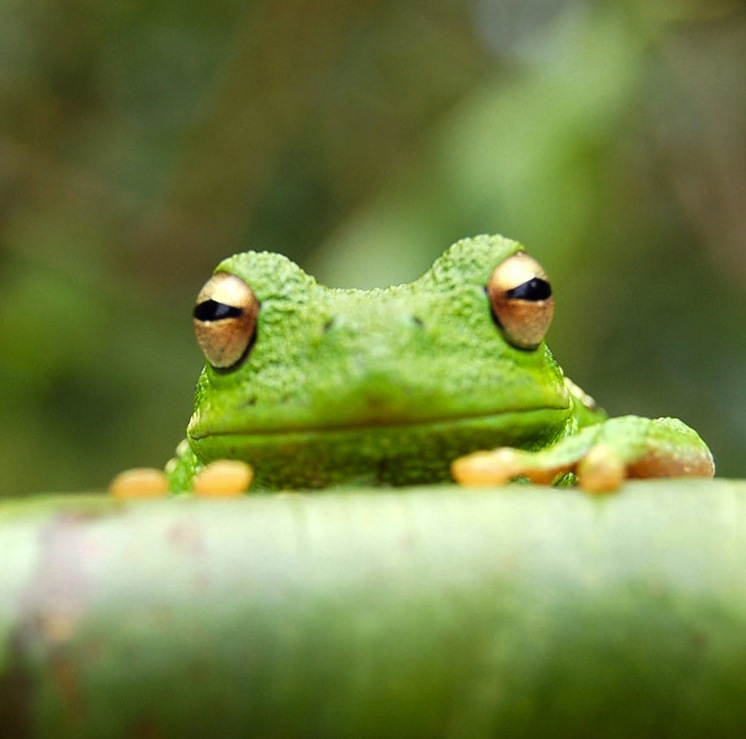
\includegraphics[width=0.5\textwidth]{frog.jpg}
% % \caption{\label{fig:frog}This is a figure caption.}
% % \end{figure}

% % \begin{table}
% % \centering
% % \begin{tabular}{l|r}
% % Item & Quantity \\\hline
% % Widgets & 42 \\
% % Gadgets & 13
% % \end{tabular}
% % \caption{\label{tab:widgets}An example table.}
% % \end{table}

% \subsection{Mathematics}

% \LaTeX{} is great at typesetting mathematics. Let $X_1, X_2, \ldots, X_n$ be a sequence of independent and identically distributed random variables with $\text{E}[X_i] = \mu$ and $\text{Var}[X_i] = \sigma^2 < \infty$, and let
% $$S_n = \frac{X_1 + X_2 + \cdots + X_n}{n}
%       = \frac{1}{n}\sum_{i}^{n} X_i$$
% denote their mean. Then as $n$ approaches infinity, the random variables $\sqrt{n}(S_n - \mu)$ converge in distribution to a normal $\mathcal{N}(0, \sigma^2)$.

% \subsection{Lists}

% You can make lists with automatic numbering \dots

% \begin{enumerate}
% \item Like this,
% \item and like this.
% \end{enumerate}
% \dots or bullet points \dots
% \begin{itemize}
% \item Like this,
% \item and like this.
% \end{itemize}

% We hope you find write\LaTeX\ useful, and please let us know if you have any feedback using the help menu above.

\end{document} to your LaTeX file where you want your
% title page.
%t
%%%%%%%%%%%%%%%%%%%%%%%%%%%%%%%%%%%%%%%%%
\title{Báo cáo đồ án cuối kỳ}
%----------------------------------------------------------------------------------------
%	PACKAGES AND OTHER DOCUMENT CONFIGURATIONS
%----------------------------------------------------------------------------------------

\documentclass[12pt]{article}
\usepackage[T5]{fontenc}
\usepackage[utf8]{inputenc}
\usepackage[vietnamese,english]{babel}
\usepackage{amsmath}
\usepackage{graphicx}
\usepackage[colorinlistoftodos]{todonotes}
\usepackage{listings}
\usepackage{hyperref}
\hypersetup{
    colorlinks=true,
    linkcolor=blue,
    filecolor=magenta,      
    urlcolor=cyan,
}


\begin{document}

\begin{titlepage}

\newcommand{\HRule}{\rule{\linewidth}{0.5mm}} % Defines a new command for the horizontal lines, change thickness here

\center % Center everything on the page
 
%----------------------------------------------------------------------------------------
%	HEADING SECTIONS
%----------------------------------------------------------------------------------------

\textsc{\LARGE Đại học Khoa học tự nhiên}\\[1.5cm] % Name of your university/college
\textsc{\Large Ngành hệ thống thông tin}\\[0.5cm] % Major heading such as course name
\textsc{\large Môn học: Máy học thống kê }\\[0.5cm] % Minor heading such as course title

%----------------------------------------------------------------------------------------
%	TITLE SECTION
%----------------------------------------------------------------------------------------

\HRule \\[0.4cm]
{ \huge \bfseries Báo cáo đồ án ứng dụng Yolo}\\[0.4cm] % Title of your document
\HRule \\[1.5cm]
 
%----------------------------------------------------------------------------------------
%	AUTHOR SECTION
%----------------------------------------------------------------------------------------

\begin{minipage}{0.4\textwidth}
\begin{flushleft} \large
\emph{Học viên:}\\
Thái Thiện -- 17C 12 031 % Your name
\end{flushleft}
\end{minipage}
~
\begin{minipage}{0.4\textwidth}
\begin{flushright} \large
\emph{Giảng viên:} \\
TS. Ngô Minh Nhựt % Supervisor's Name
\end{flushright}
\end{minipage}\\[2cm]

% If you don't want a supervisor, uncomment the two lines below and remove the section above
%\Large \emph{Author:}\\
%John \textsc{Smith}\\[3cm] % Your name

%----------------------------------------------------------------------------------------
%	DATE SECTION
%----------------------------------------------------------------------------------------

% I don't want day because it is English
% {\large \today}\\[2cm] % Date, change the \today to a set date if you want to be precise

%----------------------------------------------------------------------------------------
%	LOGO SECTION
%----------------------------------------------------------------------------------------


\includegraphics{logo/rsz_3logo-khtn.png}\\[1cm] % Include a department/university logo - this will require the graphicx package
 
%----------------------------------------------------------------------------------------

\vfill % Fill the rest of the page with whitespace

\end{titlepage}


\section{Yolo}

Trang chủ: \url{https://pjreddie.com/darknet/yolo/} 

YOLO - You Only look once - là hệ thống nhận dạng vật thể thời gian thực.

Trong đồ án này, chúng tôi sử dụng YOLOv3 

\section{Cài đặt Yolo để nhận dạng ảnh}

\subsection{Mã nguồn của tác giả YOLO}

Tác giả có hướng dẫn cách cài đặt YOLO tại trang chủ  \url{https://pjreddie.com/darknet/yolo/}. Máy tính chúng tôi dùng sử dụng hệ điều hành Ubuntu 16.04 LTS. 

Cài những thứ cần thiết để build với dòng lệnh ở lstlisting \ref{lst:buildessential}.

\begin{lstlisting}[caption={Cài những gói cần thiết để build}, label={lst:buildessential}, language=bash]
sudo apt-get build-essential
sudo apt-get install git
\end{lstlisting}

Sau đó tải mã nguồn từ Github \footnote{\url{https://github.com/pjreddie/darknet}} về build với các dòng lệnh sau (lstlisting \ref{lst:buildyolo})


\begin{lstlisting}[caption={Tải và build mã nguồn}, label={lst:buildyolo}, language=bash]
git clone https://github.com/pjreddie/darknet   
cd darknet 
make  
\end{lstlisting}

Sau đó tải model (loại lớn) \footnote{\url{https://pjreddie.com/media/files/yolov3.weights}}  huấn luyện kèm với config \footnote{\url{https://github.com/pjreddie/darknet/blob/master/cfg/yolov3.cfg}}. Ngoài ra còn có loại nhỏ (tiny) \footnote{\url{https://pjreddie.com/media/files/yolov3-tiny.weights}} và config nhỏ \footnote{\url{https://github.com/pjreddie/darknet/blob/master/cfg/yolov3-tiny.cfg}}. 

Sau đó, chạy theo ví dụ của tác giả (lstlisting \ref{lst:runexample}) hoặc theo cú pháp (lstlisting \ref{lst:runsyntax})

\begin{lstlisting}[caption={ví dụ chạy nhận diện vật thể}, label={lst:runexample}, language=bash]
./darknet detect cfg/yolov3.cfg yolov3.weights data/dog.jpg
\end{lstlisting}


\begin{lstlisting}[caption={ví dụ chạy nhận diện vật thể}, label={lst:runsyntax}, language=bash]
./darknet detect <config path> <weight path> <input image>
\end{lstlisting}


\subsection{Cài đặt YOLO bằng python}

Các tập tin python tác giả cung cấp có vẻ không tương thích với đoạn mã c++ mà chúng tôi build được ở bước trên. Vì vậy chúng tôi quyết định tìm kiếm giải pháp khác. Chúng tôi kế thừa từ mã nguồn của Ayoosh Kathuria \footnote{\url{https://github.com/ayooshkathuria/pytorch-yolo-v3}} và cải tiến cho phù hợp với nhu cầu \footnote{\url{https://github.com/ttpro1995/pytorch-yolo-v3}}.  

Yêu cầu: 
\begin{itemize}
\item python 3.6
\item Anaconda \footnote{\url{https://www.anaconda.com/download/}}
\item Pytorch \footnote{\url{https://pytorch.org/}}
\item opencv-python 
\end{itemize}

\subsubsection{Yolo Wrapper - Một lớp (class) dễ sử dụng}

Chúng tôi xây dựng một lớp YoloWrapper bao gồm hàm tạo và hàm predict để tiện việc gắn vào ứng dụng 

\paragraph{Khởi tạo}
Bước khởi tạo cần làm 3 việc: nạp danh sách lớp (từ coco.names), nạp mô hình trọng số và config. 

\paragraph{Dự đoán}
Bước dự đoán thực hiện các bước sau 

\begin{itemize}
\item Tiền xử lý: biến đổi ảnh đầu vào cho phù hợp với chiều của mạng yolo (416) 
\item Dự đoán: bỏ ma trận hình ảnh sau khi tiền xử lý vào mô hình yolo 
\item Ghi kết quả: từ kết quả dự đoán, ghi kết quả theo dạng [hình trong batch, tọa độ khung 1, tọa độ khung 2, tọa độ khung 3, tọa độ khung 4, xxx, độ tự tin, số thứ tự của tên vật thể]. Bước ghi kết quả chỉ ghi lại kết quả có độ tự tin lớn hơn threshold 
\item Scale: cái khung ở bước ghi kết quả dựa và cái hình sau khi đã biến đổi cho phù hợp với mô hình. Ta cần biến đổ nó trở lại đúng với ảnh gốc để vẽ vào ảnh gốc 
\item Vẽ khung dự đoán và tên vật thể vào ảnh gốc và trả về kết quả 
\end{itemize} 


\subsubsection{Mẫu thiết kế Singleton}

\section{Dùng Django để tạo ứng dụng web cho yolo}





Trích dẫn hình \ref{fig:node} trong đoạn chữ. 

% % Commands to include a figure:
\begin{figure}[h]
\centering

\includegraphics[width=0.5\textwidth]{image/node.PNG}
\caption{\label{fig:node} Nút}
\end{figure}


% chuong 3
\section{Chèn đoạn code}


ví dụ code \ref{lst:vdcode} là code python 


\begin{lstlisting}[caption={Đoạn code}, label={lst:vdcode}, language=python]
s = "I am Pusheen the cat"
print(s)
\end{lstlisting}

ví dụ trích dẫn \cite{robinson2013graph}


\bibliographystyle{IEEEtran}
\bibliography{bib}

%%%%%%%%%%%%%%%%%%%%%%%%%%%%%%%%%%%%%%%%%%%%%%%%%%%%
% Comments can be added to the margins of the document using the \todo{Here's a comment in the margin!} todo command, as shown in the example on the right. You can also add inline comments too:

% \todo[inline, color=green!40]{This is an inline comment.}



% \subsection{Tables and Figures}

% Use the table and tabular commands for basic tables --- see Table~\ref{tab:widgets}, for example. You can upload a figure (JPEG, PNG or PDF) using the files menu. To include it in your document, use the includegraphics command as in the code for Figure~\ref{fig:frog} below.

% % % Commands to include a figure:
% % \begin{figure}
% % \centering
% % 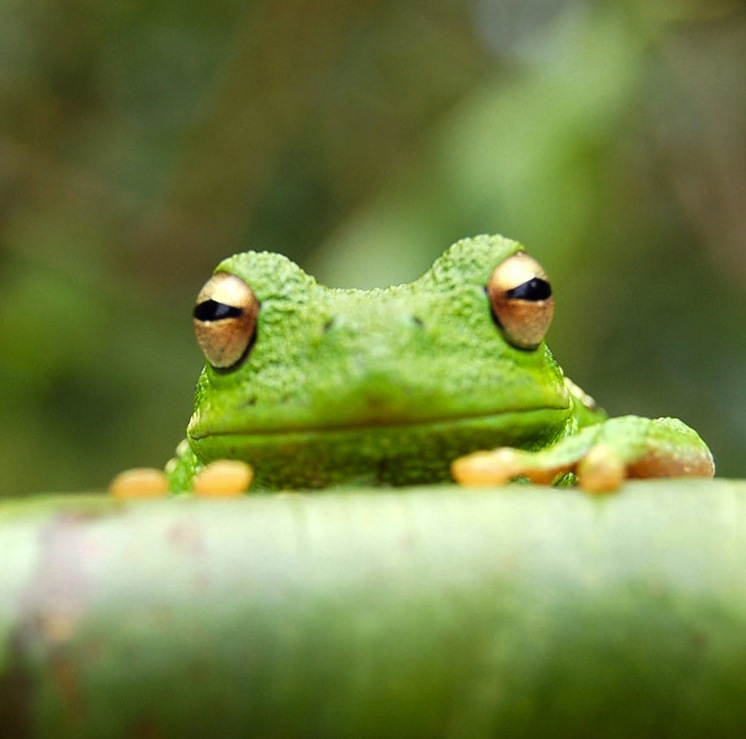
\includegraphics[width=0.5\textwidth]{frog.jpg}
% % \caption{\label{fig:frog}This is a figure caption.}
% % \end{figure}

% % \begin{table}
% % \centering
% % \begin{tabular}{l|r}
% % Item & Quantity \\\hline
% % Widgets & 42 \\
% % Gadgets & 13
% % \end{tabular}
% % \caption{\label{tab:widgets}An example table.}
% % \end{table}

% \subsection{Mathematics}

% \LaTeX{} is great at typesetting mathematics. Let $X_1, X_2, \ldots, X_n$ be a sequence of independent and identically distributed random variables with $\text{E}[X_i] = \mu$ and $\text{Var}[X_i] = \sigma^2 < \infty$, and let
% $$S_n = \frac{X_1 + X_2 + \cdots + X_n}{n}
%       = \frac{1}{n}\sum_{i}^{n} X_i$$
% denote their mean. Then as $n$ approaches infinity, the random variables $\sqrt{n}(S_n - \mu)$ converge in distribution to a normal $\mathcal{N}(0, \sigma^2)$.

% \subsection{Lists}

% You can make lists with automatic numbering \dots

% \begin{enumerate}
% \item Like this,
% \item and like this.
% \end{enumerate}
% \dots or bullet points \dots
% \begin{itemize}
% \item Like this,
% \item and like this.
% \end{itemize}

% We hope you find write\LaTeX\ useful, and please let us know if you have any feedback using the help menu above.

\end{document} to your LaTeX file where you want your
% title page.
%t
%%%%%%%%%%%%%%%%%%%%%%%%%%%%%%%%%%%%%%%%%
\title{Báo cáo đồ án cuối kỳ}
%----------------------------------------------------------------------------------------
%	PACKAGES AND OTHER DOCUMENT CONFIGURATIONS
%----------------------------------------------------------------------------------------

\documentclass[12pt]{article}
\usepackage[T5]{fontenc}
\usepackage[utf8]{inputenc}
\usepackage[vietnamese,english]{babel}
\usepackage{amsmath}
\usepackage{graphicx}
\usepackage[colorinlistoftodos]{todonotes}
\usepackage{listings}
\usepackage{hyperref}
\hypersetup{
    colorlinks=true,
    linkcolor=blue,
    filecolor=magenta,      
    urlcolor=cyan,
}


\begin{document}

\begin{titlepage}

\newcommand{\HRule}{\rule{\linewidth}{0.5mm}} % Defines a new command for the horizontal lines, change thickness here

\center % Center everything on the page
 
%----------------------------------------------------------------------------------------
%	HEADING SECTIONS
%----------------------------------------------------------------------------------------

\textsc{\LARGE Đại học Khoa học tự nhiên}\\[1.5cm] % Name of your university/college
\textsc{\Large Ngành hệ thống thông tin}\\[0.5cm] % Major heading such as course name
\textsc{\large Môn học: Máy học thống kê }\\[0.5cm] % Minor heading such as course title

%----------------------------------------------------------------------------------------
%	TITLE SECTION
%----------------------------------------------------------------------------------------

\HRule \\[0.4cm]
{ \huge \bfseries Báo cáo đồ án ứng dụng Yolo}\\[0.4cm] % Title of your document
\HRule \\[1.5cm]
 
%----------------------------------------------------------------------------------------
%	AUTHOR SECTION
%----------------------------------------------------------------------------------------

\begin{minipage}{0.4\textwidth}
\begin{flushleft} \large
\emph{Học viên:}\\
Thái Thiện -- 17C 12 031 % Your name
\end{flushleft}
\end{minipage}
~
\begin{minipage}{0.4\textwidth}
\begin{flushright} \large
\emph{Giảng viên:} \\
TS. Ngô Minh Nhựt % Supervisor's Name
\end{flushright}
\end{minipage}\\[2cm]

% If you don't want a supervisor, uncomment the two lines below and remove the section above
%\Large \emph{Author:}\\
%John \textsc{Smith}\\[3cm] % Your name

%----------------------------------------------------------------------------------------
%	DATE SECTION
%----------------------------------------------------------------------------------------

% I don't want day because it is English
% {\large \today}\\[2cm] % Date, change the \today to a set date if you want to be precise

%----------------------------------------------------------------------------------------
%	LOGO SECTION
%----------------------------------------------------------------------------------------


\includegraphics{logo/rsz_3logo-khtn.png}\\[1cm] % Include a department/university logo - this will require the graphicx package
 
%----------------------------------------------------------------------------------------

\vfill % Fill the rest of the page with whitespace

\end{titlepage}


\section{Yolo}

Trang chủ: \url{https://pjreddie.com/darknet/yolo/} 

YOLO - You Only look once - là hệ thống nhận dạng vật thể thời gian thực.

Trong đồ án này, chúng tôi sử dụng YOLOv3 

\section{Cài đặt Yolo để nhận dạng ảnh}

\subsection{Mã nguồn của tác giả YOLO}

Tác giả có hướng dẫn cách cài đặt YOLO tại trang chủ  \url{https://pjreddie.com/darknet/yolo/}. Máy tính chúng tôi dùng sử dụng hệ điều hành Ubuntu 16.04 LTS. 

Cài những thứ cần thiết để build với dòng lệnh ở lstlisting \ref{lst:buildessential}.

\begin{lstlisting}[caption={Cài những gói cần thiết để build}, label={lst:buildessential}, language=bash]
sudo apt-get build-essential
sudo apt-get install git
\end{lstlisting}

Sau đó tải mã nguồn từ Github \footnote{\url{https://github.com/pjreddie/darknet}} về build với các dòng lệnh sau (lstlisting \ref{lst:buildyolo})


\begin{lstlisting}[caption={Tải và build mã nguồn}, label={lst:buildyolo}, language=bash]
git clone https://github.com/pjreddie/darknet   
cd darknet 
make  
\end{lstlisting}

Sau đó tải model (loại lớn) \footnote{\url{https://pjreddie.com/media/files/yolov3.weights}}  huấn luyện kèm với config \footnote{\url{https://github.com/pjreddie/darknet/blob/master/cfg/yolov3.cfg}}. Ngoài ra còn có loại nhỏ (tiny) \footnote{\url{https://pjreddie.com/media/files/yolov3-tiny.weights}} và config nhỏ \footnote{\url{https://github.com/pjreddie/darknet/blob/master/cfg/yolov3-tiny.cfg}}. 

Sau đó, chạy theo ví dụ của tác giả (lstlisting \ref{lst:runexample}) hoặc theo cú pháp (lstlisting \ref{lst:runsyntax})

\begin{lstlisting}[caption={ví dụ chạy nhận diện vật thể}, label={lst:runexample}, language=bash]
./darknet detect cfg/yolov3.cfg yolov3.weights data/dog.jpg
\end{lstlisting}


\begin{lstlisting}[caption={ví dụ chạy nhận diện vật thể}, label={lst:runsyntax}, language=bash]
./darknet detect <config path> <weight path> <input image>
\end{lstlisting}


\subsection{Cài đặt YOLO bằng python}

Các tập tin python tác giả cung cấp có vẻ không tương thích với đoạn mã c++ mà chúng tôi build được ở bước trên. Vì vậy chúng tôi quyết định tìm kiếm giải pháp khác. Chúng tôi kế thừa từ mã nguồn của Ayoosh Kathuria \footnote{\url{https://github.com/ayooshkathuria/pytorch-yolo-v3}} và cải tiến cho phù hợp với nhu cầu \footnote{\url{https://github.com/ttpro1995/pytorch-yolo-v3}}.  

Yêu cầu: 
\begin{itemize}
\item python 3.6
\item Anaconda \footnote{\url{https://www.anaconda.com/download/}}
\item Pytorch \footnote{\url{https://pytorch.org/}}
\item opencv-python 
\end{itemize}

\subsubsection{Yolo Wrapper - Một lớp (class) dễ sử dụng}

Chúng tôi xây dựng một lớp YoloWrapper bao gồm hàm tạo và hàm predict để tiện việc gắn vào ứng dụng 

\paragraph{Khởi tạo}
Bước khởi tạo cần làm 3 việc: nạp danh sách lớp (từ coco.names), nạp mô hình trọng số và config. 

\paragraph{Dự đoán}
Bước dự đoán thực hiện các bước sau 

\begin{itemize}
\item Tiền xử lý: biến đổi ảnh đầu vào theo phương pháp letterbox cho phù hợp với chiều của mạng yolo (416) 
\item Dự đoán: bỏ ma trận hình ảnh sau khi tiền xử lý vào mô hình yolo 
\item Ghi kết quả: từ kết quả dự đoán, ghi kết quả theo dạng [hình trong batch, tọa độ khung 1, tọa độ khung 2, tọa độ khung 3, tọa độ khung 4, xxx, độ tự tin, số thứ tự của tên vật thể]. Bước ghi kết quả chỉ ghi lại kết quả có độ tự tin lớn hơn threshold 
\item Scale: cái khung ở bước ghi kết quả dựa và cái hình sau khi đã biến đổi cho phù hợp với mô hình. Ta cần biến đổ nó trở lại đúng với ảnh gốc để vẽ vào ảnh gốc 
\item Vẽ khung dự đoán và tên vật thể vào ảnh gốc và trả về kết quả 
\end{itemize} 

Công thức để scale hình ban đầu về  kích thước cho mô hình. Đầu tiên hình $h_0, w_0$ sẽ được scale về đúng tỉ lệ thành $h_1, w_1$, sau đó sẽ được padding để có kích thước theo chuẩn của model $h, w$
% new_h = int(img_h * min(w/img_w, h/img_h))

\begin{equation}
    h_1 = h_0 * min(\frac{w}{w_0}, \frac{h}{h_0})   
\end{equation}

\begin{equation}
    w_1 = w_0 * min(\frac{w}{w_0}, \frac{h}{h_0})   
\end{equation}

Công thức để scale khung về đúng ban đầu 

\begin{equation}
    scaling\_horizontal = \frac{inp\_dim}{im\_dim_0}  
\end{equation}

\begin{equation}
    scaling\_vertical = \frac{inp\_dim}{im\_dim_1}
\end{equation}

\begin{equation}
    scaling\_factor = min(scaling\_horizontal, scaling\_vertical)
\end{equation}


\begin{equation}
    output_{1,3} = output_{1,3} - \frac{inp\_dim - scaling\_factor * im\_dim_0 }{2} 
\end{equation}

\begin{equation}
    output_{2,4} = output_{2,4} - \frac{inp\_dim - scaling\_factor * im\_dim_1 }{2} 
\end{equation}

\begin{equation}
    output_{1,3} = \frac{output_{1,3}}{scaling\_factor}  
\end{equation}

\begin{equation}
    output_{2,4} = \frac{output_{2,4}}{scaling\_factor}  
\end{equation}

\subsubsection{Mẫu thiết kế Singleton}



\section{Dùng Django để tạo ứng dụng web cho yolo}





Trích dẫn hình \ref{fig:node} trong đoạn chữ. 

% % Commands to include a figure:
\begin{figure}[h]
\centering

\includegraphics[width=0.5\textwidth]{image/node.PNG}
\caption{\label{fig:node} Nút}
\end{figure}


% chuong 3
\section{Chèn đoạn code}


ví dụ code \ref{lst:vdcode} là code python 


\begin{lstlisting}[caption={Đoạn code}, label={lst:vdcode}, language=python]
s = "I am Pusheen the cat"
print(s)
\end{lstlisting}

ví dụ trích dẫn \cite{robinson2013graph}


\bibliographystyle{IEEEtran}
\bibliography{bib}

%%%%%%%%%%%%%%%%%%%%%%%%%%%%%%%%%%%%%%%%%%%%%%%%%%%%
% Comments can be added to the margins of the document using the \todo{Here's a comment in the margin!} todo command, as shown in the example on the right. You can also add inline comments too:

% \todo[inline, color=green!40]{This is an inline comment.}



% \subsection{Tables and Figures}

% Use the table and tabular commands for basic tables --- see Table~\ref{tab:widgets}, for example. You can upload a figure (JPEG, PNG or PDF) using the files menu. To include it in your document, use the includegraphics command as in the code for Figure~\ref{fig:frog} below.

% % % Commands to include a figure:
% % \begin{figure}
% % \centering
% % 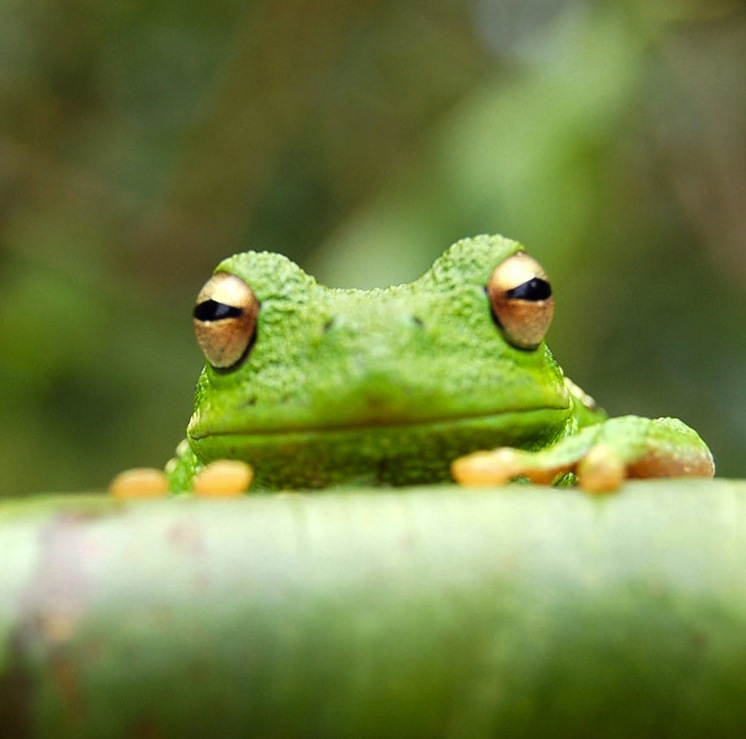
\includegraphics[width=0.5\textwidth]{frog.jpg}
% % \caption{\label{fig:frog}This is a figure caption.}
% % \end{figure}

% % \begin{table}
% % \centering
% % \begin{tabular}{l|r}
% % Item & Quantity \\\hline
% % Widgets & 42 \\
% % Gadgets & 13
% % \end{tabular}
% % \caption{\label{tab:widgets}An example table.}
% % \end{table}

% \subsection{Mathematics}

% \LaTeX{} is great at typesetting mathematics. Let $X_1, X_2, \ldots, X_n$ be a sequence of independent and identically distributed random variables with $\text{E}[X_i] = \mu$ and $\text{Var}[X_i] = \sigma^2 < \infty$, and let
% $$S_n = \frac{X_1 + X_2 + \cdots + X_n}{n}
%       = \frac{1}{n}\sum_{i}^{n} X_i$$
% denote their mean. Then as $n$ approaches infinity, the random variables $\sqrt{n}(S_n - \mu)$ converge in distribution to a normal $\mathcal{N}(0, \sigma^2)$.

% \subsection{Lists}

% You can make lists with automatic numbering \dots

% \begin{enumerate}
% \item Like this,
% \item and like this.
% \end{enumerate}
% \dots or bullet points \dots
% \begin{itemize}
% \item Like this,
% \item and like this.
% \end{itemize}

% We hope you find write\LaTeX\ useful, and please let us know if you have any feedback using the help menu above.

\end{document}